\documentclass[fleqn,10pt,lineno]{olplainarticle}
% Use option lineno for line numbers

\graphicspath{{./figures/}}

\usepackage[implicit=false]{hyperref}

\title{Assessing United States county-level exposure for tropical cyclone impact
research}

\author[a,1]{G. Brooke Anderson} 
\author[a,b]{Joshua Ferreri}
\author[c]{Mohammad Al-Hamdan} 
\author[c]{William Crosson} 
\author[d]{Andrea Schumacher} 
\author[e]{Seth Guikema} 
\author[f]{Steven Quiring} 
\author[g]{Dirk Eddelbuettel} 
\author[a]{Meilin Yan} 
\author[h]{Roger D. Peng}

\affil[a]{Department of Environmental \& Radiological Health Sciences, Colorado 
  State University, Fort Collins, CO, 80523} 
\affil[b]{University of Colorado Denver School of Medicine, Aurora, CO, 80045} 
\affil[c]{Universities Space Research Association, NASA Marshall Space Flight 
  Center, Huntsville, AL, 35805}
\affil[d]{Cooperative Institute for Research in the Atmosphere, Colorado State
  University, Fort Collins, CO, 80523} 
\affil[e]{Department of Industrial and Operations Engineering, University of 
  Michigan, Ann Arbor, MI, 48109}
\affil[f]{Department of Geography, Ohio State University, Columbus, OH, 43210}
\affil[g]{Debian and R Projects; Department of Statistics, University of
  Illinois at Urbana-Champaign, Champaign, IL, 61820} 
\affil[h]{Department of Biostatistics, Johns Hopkins Bloomberg School of Public 
  Health, Baltimore, MD, 21205}

\keywords{Hurricanes, Tropical cyclones, Disaster impacts, Exposure assessment}

\begin{abstract} Hurricanes and other tropical cyclones bring severe impacts to
U.S. communities. These impacts can result from a variety of storm-related
hazards, including extreme wind, rain, flooding, and tornadoes. Impact studies
vary widely in how they classify exposure to tropical cyclones, using various
hazard-based metrics and, in some cases, using distance from the storm as a
surrogate for exposure to storm-related hazards. Here we measure county-level
exposure to tropical cyclones in the United States based on distance from the
storm, maximum sustained wind, rainfall, flooding, and tornadoes for all
land-falling or near-land Atlantic basin storms for 1988--2015. We show that the
locations identified as storm-exposed varied substantially when switching among
these metrics. For example, most wind-based storm exposures were limited to
southern counties near the coast, while flood- and rain-based exposures often
extended to inland and northern counties. We also show that distance to the
storm served as, at best, a moderate, and often a poor, surrogate in identifying
exposure to storm-related wind, rain, floods, or tornadoes. Therefore, when
impact studies use distance as a surrogate for tropical cyclone exposures or use
one hazard-based metric (e.g., wind-based) when the impact is partly or fully
caused by a different storm hazard, the analysis will be prone to exposure
misclassification, which can mask true associations, even strong associations.
To facilitate future research, we make this multi-hazard storm exposure data
available through open-source software.  \end{abstract}

\begin{document}

\flushbottom 
\maketitle 
\thispagestyle{empty}

\section*{Introduction}

Tropical cyclones, including hurricanes, can have disasterous impacts in the
United States (U.S.). A tropical cyclone's high winds can bring health risks
and property damage caused by structural damage of houses and other buildings,
falling trees, and wind-borne debris \citep{rappaport2000} and 
cause power outages \citep{liu2005, han2009}, introducing a number of
threats to human and ecological health, including water quality
risks if the outage affects wastewater treatment plants \citep{mallin2006}.
Other risks can exist without severe wind; for example, one study found that
most of the direct hurricane-related deaths in the U.S. between 1970 and 1999
occurred in cases when wind was below hurricane strength, including for
Tropical Storms Charley in 1998 and Alberto in 1994 \citep{rappaport2000}.
Tropical cyclones can produce excessive rain, especially in certain
topographies (e.g., near mountains), so counties well inland sometimes
experience more extreme rain than coastal counties. Flood risks from tropical
cyclones can result from this rain, although the two risks are not perfectly
correlated \citep{chen2015}. In the U.S., over half of hurricane-related direct
deaths from 1970 to 1999 from Atlantic basin storms were a result of freshwater
flooding \citep{rappaport2000}. Flooding can also degrade water quality
\citep{mallin2006}, which can threaten both human and ecological health.


To measure tropical cyclone exposure for either investigations of exposure
patterns or for estimation of storm impacts, including health impacts, studies
have varied widely in how they determine storm exposure (some examples shown in
Fig. S1). While many studies have measured exposure based on specific hazards
of the storm (e.g., wind, rain), many studies have used distance from the
storm's central track as a surrogate in identifying exposure to the hazards of
a storm (Fig. S1) (e.g., \citep{czajkowski2011, tansel2010, kinney2008,
caillouet2008increase}). Distance from the storm's central track can be easily
measured using widely-available hurricane tracking data. There are, however, a
number of limitations to using distance to assess exposure to tropical
cyclones, and there are reasons to suspect that exposure classifications based
on other storm hazards may disagree with distance-based classifications.
Tropical cyclones vary dramatically in size: U.S. storms have been observed
with radii to maximum winds as small as 20 kilometers and as large as 200
kilometers \citep{mallin2006, quiring2011variations}. While a number of storm
hazards are strongly associated with distance from the storm's center (e.g.,
wind and, at the coast, storm surge and waves \citep{rappaport2000, kruk2010}),
other hazards like dangerous rain, floods, and tornadoes can occur well away
from the storm's central track \citep{rappaport2000, atallah2007, moore2012}.
For example, fatal tropical cyclone tornadoes, which were linked to over 300
deaths in the U.S.  between 1995 and 2009, most often occur 200--500 kilometers
from the storm's center \citep{moore2012}. Further, distance-based exposure
metrics that use buffers tend to use an equal buffer distance on each side of
the storm track (e.g., \citep{czajkowski2011, grabich2015, grabich2016,
zandbergen2009, tansel2010}), but the forces of a storm tend to be distributed
around the center in a non-symmetrical way. For example, extreme winds are more
common to the right of the track where counter-clockwise cyclonic winds move in
concert with the storm's forward motion \citep{halverson2015}, and the fatal
tornadoes associated with U.S. tropical cyclones between 1995 and 2009 occurred
almost exclusively to the right of the storm's track, mostly in the right-front
quandrant (northeast) of the storm \citep{moore2012}. Rain, conversely, is
often heaviest to the left of the storm's track, especially when the storm
interacts with other weather systems \citep{atallah2003, atallah2007,
zhu2013variations} or undergoes an extratropical transition
\citep{elsberry2002}.

The use of different exposure metrics across studies hampers the development of
a scientific consensus on storm-related risks, as differences observed between
studies could result from differences in exposure assessment.  Further, if a
study misclassifies exposure to the storm hazard or hazards that cause an
impact, estimates of storm risks or impacts will be biased, making it hard to
identify true associations. These concerns are particularly important if there
are large differences in the locations that are determined to be storm-exposed
based on different metrics.  To investigate this, we measured county-level
exposure to tropical cyclones in all eastern United States counties using five
metrics (Table \ref{tab:exposuremetrics}): (1) distance to storm track; (2)
maximum sustained wind speed; (3) cumulative rainfall; (4) flood events; and
(5) tornado events.  We assessed exposure at the county level since data on
many potential impacts are available at county-level aggregations (e.g., direct
hurricane-related deaths \citep{czajkowski2011}; birth outcomes
\citep{grabich2015, grabich2016}; autism prevalence \citep{kinney2008}) and
since decisions and policies to prepare for, and respond to, storms are often
undertaken at the county level \citep{zandbergen2009, rappaport2000}. We
measured how well exposure classification agreed across these five metrics in
terms of classifying individual counties as exposed to a storm.  Finally, to
make this hazard-specific tropical cyclone exposure data available to other
researchers, we published open source software for county-based hurricane
exposure assessment in U.S. counties \citep{hurricaneexposure}.

\begin{table}%[tbhp] 
\centering 
\caption{Exposure metrics considered to assess county-level exposure to 
tropical cyclones}
\begin{tabular}{p{0.9cm}p{2.5cm}p{9cm}} 
Metric & Available & Criteria for exposure \\ \midrule 
Distance & 1988--2015 & County population mean center within 100 kilometers of storm track \\ 
Rain & 1988--2011 & County cumulative rainfall of 75 millimeters or more over the period from two days before to one day after the storm's closest approach and county population mean center within 500 kilometers of the storm track \\ 
Wind & 1988--2015 & Modeled maximum sustained wind speed at the county's population mean center 15 meters per second or higher during the storm\\ 
Flood & 1996--2015 & Flood event listed in the National Oceanic and Atmospheric Administration (NOAA) Storm Events database for the county with a start date within two days of the storm's closest approach and county population mean center within 500 kilometers of the storm track \\
Tornado & 1996--2015 & Tornado event listed NOAA Storm Events database for the county with a start date within two days of the storm's closest approach and county population mean center within 500 kilometers of the storm track\\
\bottomrule 
\end{tabular} 
\label{tab:exposuremetrics} 
\end{table}

\section*{Methods and Materials}
,
All counties in the eastern half of the U.S. (e.g., Fig.
\ref{fig:averageexposure}), as of the 2010 U.S. Decennial Census, were included
in the study. The study covered all tracked storms in the revised Atlantic
hurricane database (HURDAT2 \citep{landsea2013}) and that came within 250
kilometers of at least one study county between 1988 and 2015 (Fig. S2). HURDAT2
is a post-storm assessment of each storm conducted by the U.S. National
Hurricane Center (NHC) and incorporates data from a variety of sources,
including satellite data and, when available, aircraft reconnaisance data
\citep{landsea2013, jarvinen1988}. These data typically give measurements of
storm center location at 6-hour intervals, at synoptic times (i.e., 6:00 am,
12:00 pm, 6:00 pm, and 12:00 am UTC); some landfalling storms have an additional
observation at the time of landfall \citep{landsea2013}.

\subsection*{Distance-based exposure metric.}

For the rain-based exposure metric, cumulative rainfall was estimated for the
period from two days before to one day after the date of a storm's closest
approach to a county. Daily county-level rainfall was determined by aggregating
hourly, 1/8 degree gridded reanalysis data from the North American Land Data
Assimilation System Phase 2 (NLDAS-2) precipitation data files
\citep{rui2013nldas}. The NLDAS-2 data integrate satellite-based and land-based
monitoring and applies a land-surface model to create a reanalysis dataset that
is spatially and temporally complete across the continental U.S.
\citep{rui2013nldas, alhamdan2014environmental}. These data have been used in
previous research to investigate tropical cyclones (e.g., \citep{chen2015}). To
aggregate to county-level, hourly data at each grid point were summed to create
a daily sum and these grid-point specific rainfall totals were then averaged
across all grid points within a county's 1990 U.S. Census boundaries to create a
county-level daily total \citep{alhamdan2014environmental, cdcwonder}. This
county-level precipitation data are publicly available through the U.S. Centers
for Disease Control's Wide-ranging Online Data for Epidemiological Research
(WONDER) database \citep{cdcwonder, alhamdan2014environmental}. The
rainfall-based exposure metric was only available for storms through 2011, the
period for which the reanalysis rainfall data aggregated to county-level daily
totals was available \citep{cdcwonder, alhamdan2014environmental}. Validation
analysis of this and other hazard-based exposure data is given in the Supporting
Information.

\subsection*{Wind-based exposure metric}

Ground-based observations of wind speed are problematic during storms, as
instruments often fail at high wind speed, while reanalysis data, often
available at hourly or higher resolution, can be too smooth to capture wind
extremes associated with a storm. Therefore, to create a dataset of county-level
sustained winds during historical storms, we modeled maximum sustained wind
speeds at each county's population mean center \citep{countycenters}. HURDAT2
Best Track data were interpolated from 6-hourly reported values to 15-minute
increments using natural cubic splines \citep{stormwindmodel}, and then
sustained wind speed was modeled for each county center at each 15-minute
increment using a double exponential wind speed model
\citep{willoughby2006parametric} to estimate maximum ground-level sustained wind
speed at each county center \citep{stormwindmodel}. Asymmetry in wind speeds
around the storm center was incorporated into the wind speed model
\citep{phadke2003modeling, stormwindmodel}. The maximum value of this modeled
wind speed was determined for each county as the maximum windspeed across the
15-minute incremented modeled values throughout the storm.

\subsection*{Flood- and tornado-based exposure metrics}

To identify flood- and tornado-based exposures to tropical cyclones in U.S.
counties, we used event listings from the National Oceanic and Atmospheric
Administration (NOAA)'s Storm Event Database \citep{stormevents}. For each
storm, we identified all events with event types related to flooding (``Flood",
``Flash Flood", ``Coastal Flood") and tornadoes (``Tornado") and that occurred
in a county within 500 kilometers of the storm's track and within a five-day
window centered on the date of the storm's closest approach to the county
\citep{hurricaneexposuredata}. ``Flood", ``Flash Flood" and ``Tornado" events in
this database were reported by county Federal Information Processing Standard
(FIPS) code. ``Coastal Flood" events were reported by forecast zone; for these,
the event was matched to the appropriate county if possible
\citep{noaastormevents}. While this database has recorded storm data since 1950,
its coverage changed substantially in 1996 to cover a wider variety of storm
events \citep{stormevents}. We therefore only considered these metrics of
hurricane exposure for storms in 1996 and later.

\subsection*{Assessing agreement in exposure classification across exposure
metrics}

Two of the exposure metrics (flood- and tornado-based) were inherently binary;
for the other exposure metrics, each county was classified as exposed to a storm
based on whether the continuously-measured exposure metric exceeded a certain
threshold (Table \ref{tab:exposuremetrics}). We assessed county-level tropical
cyclone exposure in the eastern U.S. based on each exposure metrics (Table
\ref{tab:exposuremetrics}) for all land-falling or near-land Atlantic basin
storms. Depending on available exposure data, this assessment included some or
all of the period from 1988 to 2015, a period with 136 tropical cyclones that
made U.S. landfall or passed within 250 kilometers (155 miles) of at least one
U.S. county (Fig. S2).

We then measured agreement between exposure metrics in the classification of a
county as exposed or unexposed to a specific storm. For this measurement, we
calculated the within-storm Jaccard index \citep{jaccard1901distribution,
jaccard1908nouvelles} between every pair-wise combination of hazard metrics.
The Jaccard index ($J_s$) measures similarity between two metrics ($X_{1,s}$
and $X_{2,s}$) for storm $s$ as the proportion of counties in which both of the
metrics classify the county as exposed out of all counties classified as
exposed by at least one of the metrics:

\begin{equation} 
J_s = \frac{X_{1,s} \cap X_{2,s}}{X_{1,s} \cup X_{2,s}}
\end{equation}

This metric can range from 0, in the case of no overlap between the counties
classified as ``exposed" based on the two metrics, to 1, in the case that the
two metrics classify exactly the same counties as ``exposed" to the storm.

\section*{Results}

\begin{figure*}%[tbhp] 
\centering 
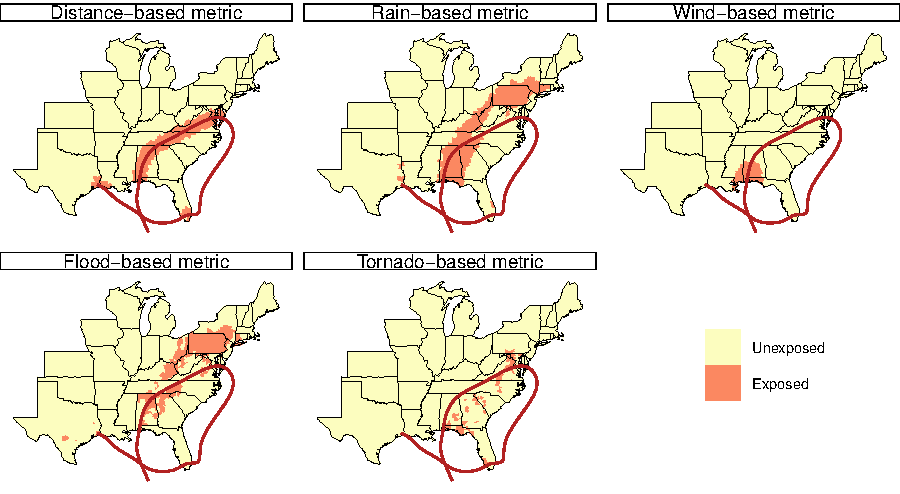
\includegraphics[width=16cm]{ivanonly}
\caption{Counties classified as exposed to Hurricane Ivan (2004) under each
exposure metric (Table 1). The red line shows the track of Hurricane Ivan 
based on the revised Atlantic hurricane database (HURDAT2 \citep{landsea2013}).
Similar maps for other large-extent storms are given in Fig. S5.}
\label{fig:ivanexposure} 
\end{figure*}

\subsection*{Patterns in tropical cyclone exposures in eastern U.S. counties}

Table [x] provides summary statistics on ...  Table [x] includes some measures
of the number of counties exposed to the storm based on each exposure metric
(Tab. [x]) Median storm extent was largest when exposure was classified based
on distance (median storm extent: 62 counties exposed). The measured extent of
storms also tended to be higher when using exposure metrics based on rain
(median: 21 counties exposed) or wind (median: 26 counties exposed) versus
based on floods (median: 9 counties exposed) or tornadoes (median: 1 county
exposed).  For every metric except the tornado-based metric, we identified at
least one storm with over 300 counties exposed. However, the largest-extent
storm varied by metric (e.g., Beryl [1994] exposed the most counties based on
distance, Frances [2004] based on rain, and Ike [2008] based on wind).

\subsection*{County-specific exposure classification}

\begin{figure}%[tbhp] 
\centering 
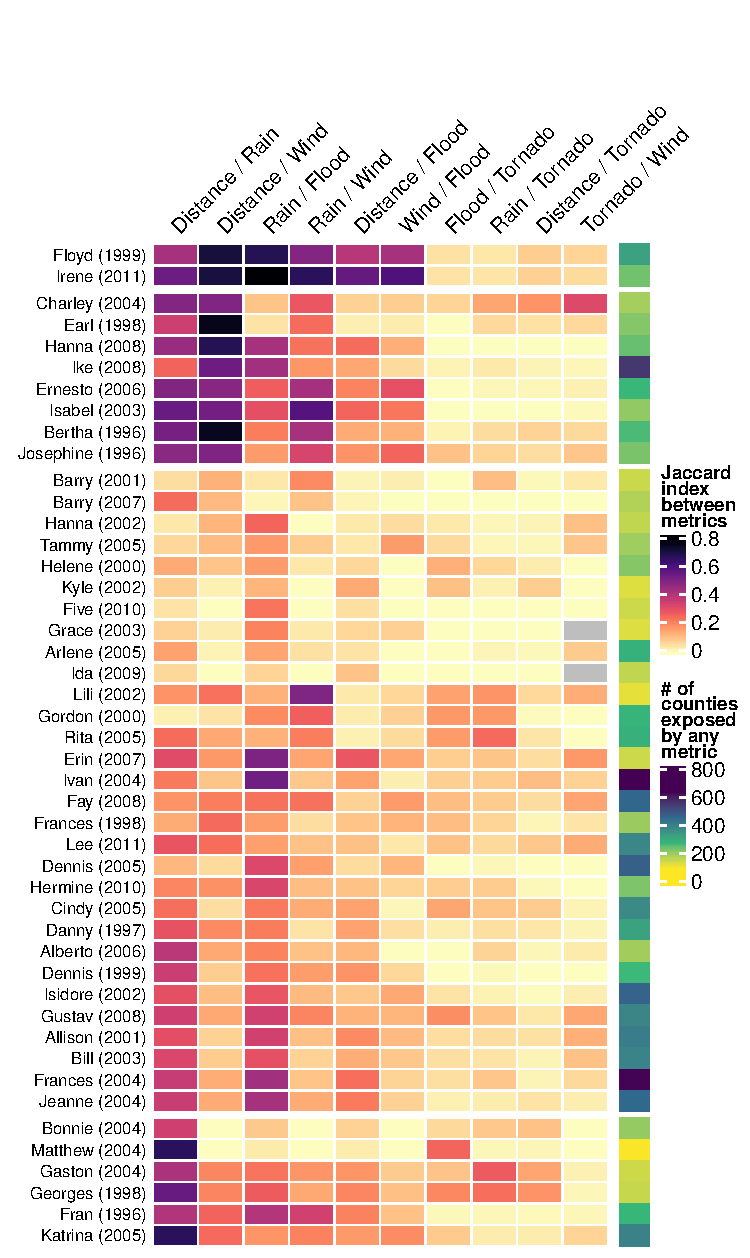
\includegraphics[width = 0.7\linewidth]{jaccard_heatmap} 
\caption{Heatmap of Jaccard index values for
specific exposure metric pairs within storms. Only storms between 1996 and 2011,
and for which at least 250 counties were exposed based on at least one metric,
are included. The color of each cell within the main heatmap indicates the value
of the Jaccard index (proportion of counties classified as exposed by both
metrics out of storms classified as exposed by either metric) for a given pair
of metrics for a given storm. Storms are displayed within clusters that have
similar patterns in county-level exposure agreement for metric pairs, based on
hierarchical clustering using the complete link method
\citep{murtagh2012algorithms} (i.e., storms in the same cluster tend to have
similar patterns for the pairwise strength of agreement among metrics); columns
are also ordered based on hierarchical clustering. The colors to the right of
the main heatmap for each storm indicate the total number of counties classified
as exposed to the storm by any of the five metrics, providing an estimate of
storm extent. Maps are available showing the counties identified as exposed
under each of five metrics for the widest-extent storm in each cluster:
Hurricane Ivan (2004) (Fig. \ref{fig:ivanexposure}) and Hurricanes Floyd (1999),
Lee (2011), Cindy (2005), and Katrina (2005) (Fig. S5).} 
\label{fig:jaccard}
\end{figure}

We found that switching among these metrics typically resulted in large
differences in which counties were identified as exposed to a particular storm.
Fig. \ref{fig:ivanexposure} gives an example for Hurricane Ivan (2004), a
record-breaking storm in terms of its duration as a major hurricane
\citep{franklin2006atlantic}. When county-level exposure was determined based on
the wind metric, only counties near two of the storm's landfalls were assessed
as exposed. For rain- and flood-based metrics, however, exposure extended to the
left of the track, including counties as far north as New York and Connecticut,
while for the tornado metric, exposed counties tended to be to the right of the
track and included several counties in central North Carolina, South Carolina,
and Georgia that were not identified as exposed to Ivan based on any other
metric.

We drew similar conclusions when we investigated all 46 storms between 1996 and
2011 (the period for which all five metrics were available) for which 250 or
more counties were exposed based on at least one metric (Fig.
\ref{fig:jaccard}). The tornado-based metric showed universally poor agreement
with other metrics in county-level classification across all storms considered.
For other pairs of metrics, there were also generally large differences in
which counties were determined to be exposed to the storm, with the Jaccard
index values (see Methods) below 0.4 for most metric pairs in most storms.

There were, however, a few exceptions---storms in which similar counties were
determined to be exposed to the storm for two or more of the metrics
considered.  For Floyd (1999) and Irene (2011), for example, county-level
classification agreed moderately to well (Jaccard index of approximately
0.5--0.8) for all pairs of exposure metrics except those including the
tornado-based metric. These storms both made their first U.S. landfall in North
Carolina at minor hurricane windspeeds (Category 2 and 1, respectively) and
then skimmed the eastern coast of the U.S. north through New England, bringing
large rainfall to much of the eastern coast from North Carolina north and
causing extensive inland flooding in North Carolina (Floyd) and New England
(Irene) \citep{avila2013atlantic, lawrence2000atlantic}. For another set of
storms (e.g., Lee [2011], Ernesto [2006], and Bertha [1996]), there was
moderate to good agreement for all pairwise combinations of distance, rain, and
wind, but poor agreement for all other combinations of metrics. Most of these
storms either skimmed along the eastern coast north of North Carolina (Bertha
[1996], Charley [2004], Gaston [2004], Barry [2007], Hanna [2008]), in a
pattern similar to Hurricanes Floyd (1999) and Irene (2011), or made landfall
in or near the Florida panhandle and cut across to exit into the Atlantic
around North Carolina (Josephine [1996], Earl [1998], Alberto [2006]). However,
these two sets of storms represented the minority of all storms considered; for
most of the storms, there was low overlap in the counties determined to be
exposed to the storm for most pairings of metrics.

\begin{figure*}%[tbhp] 
\centering
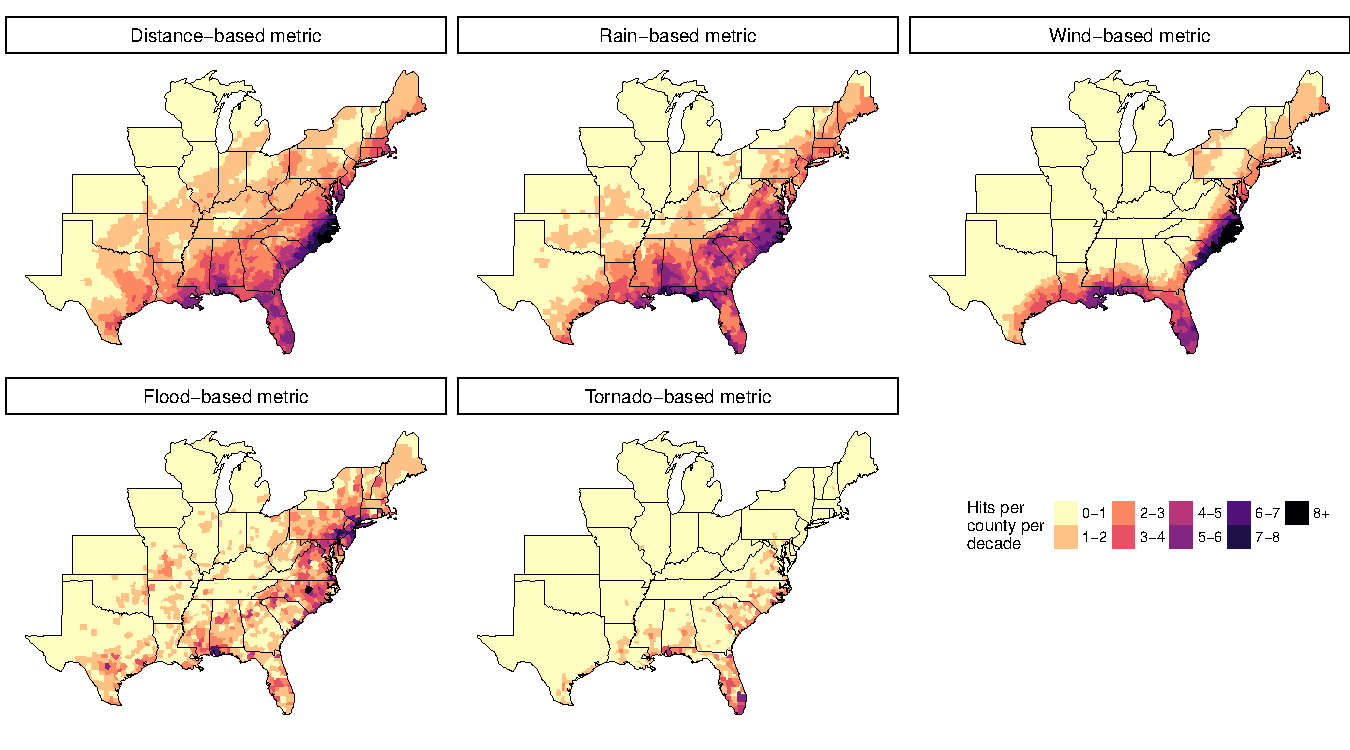
\includegraphics[width=16cm]{averageexposureonly} 
\caption{Average number of storm exposures per decade in U.S. counties for 
each exposure metric. The criteria behind each of the five metrics is given 
in Table \ref{tab:exposuremetrics}. The years used to estimate these averages 
are based on years of available exposure data (distance and wind: 1988--2015; 
rain: 1988--2011; flood and tornado: 1996--2015). Similar patterns persist when
analysis is restricted to years with all exposure data available (1996--2011;
Fig. S3).} 
\label{fig:averageexposure} 
\end{figure*}

\subsection*{Geographic patterns in tropical cyclone exposures}

When different metrics were used to assess average tropical cyclone exposure in
U.S. counties, geographic patterns varied substantially; in fact, some areas of
the U.S. that experienced regular exposures to storm-related excessive rainfall
and floods were not identified as areas of regular risk based on more commonly
used assessment metrics like wind or distance (Figs. \ref{fig:averageexposure},
S3). Wind-based exposure had a strong coastal pattern, with almost all
exposures in counties within about 200 kilometers (124 miles) of the coastline,
mostly in eastern North and South Carolina, southern Florida, and the area near
the outlet of the Mississippi River. While exposures by rain- and
distance-based metrics were also more common in coastal areas compared to
inland areas, inland exposures were much more common based on these two metrics
compared to the wind-based metric. Rain and, to some extent, flood exposures
were characterized by a pattern defined by the Appalachian Mountains, with much
lower exposures west of the mountain range than to the east.  Flood- and,
especially, tornado-based exposures were much less common than exposures based
on other metrics. Almost all tornado-based exposures were in coastal states,
with most in Florida, Alabama, South Carolina, and North Carolina and almost
none north of Maryland. Flood-based exposures were highest in North Carolina
and along the South Carolina coast, as well as further north in New Jersey,
southeastern Pennsylvania, and southeastern New York.

We have included a case study in the Supporting Information showing how these
differences can strongly influence estimates of which U.S. counties have the
largest expected physical exposure to tropical cyclones among a susceptible
subpopulation, Medicare beneficiaries who are reliant on electricity for
medical equipment \citep{empower}.

\subsection*{Software}

To assist with future tropical cyclone impact studies, we created and published
open source software that includes the hazard-specific, county-level tropical
cyclone data in this paper, as well as tools to explore and map that data
\citep{hurricaneexposure, hurricaneexposuredata}.  We investigated how well
these data correspond with data from other available sources (Figs. S6--8).
While generally in agreement with data from other sources, there are a few
limitations. The wind data are based on modeled, rather than observed, values,
and while the modeled wind data generally agree well with post-analyis maximum
wind radii from the revised Atlantic hurricane database (HURDAT2
\citep{landsea2013}) (Fig. S6), for a few storms it did not (e.g., Fig.  S9).
The rainfall data are from re-analysis data, which are generally
well-correlated with observed ground-based station data but may oversmooth
extreme measurements (Fig. S7).  

\section*{Discussion}

Tropical cyclones impact public health in many ways, and epidemiological studies
of the health impacts of tropical cyclone exposures could help improve
preparedness for and response to future storms. However, tropical storms are
multi-hazard events, making it more complicated to measure exposure to tropical
cyclones compared to other weather exposures like temperature and precipitation.
... Our results can inform exposure assessment for future county-level studies
of the health impacts of tropical cyclones exposures, and the data and software
presented provides multi-hazard, county-level exposure data for multiple
tropical cyclone hazards for such studies.

Wind-based exposure had a strong coastal pattern, with almost all exposures in
counties within about 200 kilometers (124 miles) of the coastline, mostly in
eastern North and South Carolina, southern Florida, and the area near the
outlet of the Mississippi River. This is consistent with the dramatic decrease
in wind intensity that typically characterizes the landfall of tropical
cyclones. While exposures by rain- and distance-based metrics were also more
common in coastal areas compared to inland areas, inland exposures were much
more common based on these two metrics compared to the wind-based metric. Rain
and, to some extent, flood exposures were characterized by a pattern defined by
the Appalachian Mountains, with much lower exposures west of the mountain range
than to the east. This agrees with previous research indicating that the
Appalachian mountains' topography both enhances precipitation during tropical
cyclones and provides hydrological conditions for severe flooding
\citep{rees2001}.  Almost all tornado-based exposures were in coastal states,
with most in Florida, Alabama, South Carolina, and North Carolina and almost
none north of Maryland. This pattern may be linked with previous findings that
most noteworthy storm-related tornadoes occur on the right-side of the storm
track in Atlantic Basin U.S. storms \citep{moore2012}.

The tropical cyclone exposure averages shown in Fig. \ref{fig:averageexposure}
are limited as estimates of long-term frequencies, as tropical cyclones follow
decadal patterns \citep{kossin2007more} likely not adequately captured in the
available data. However, these frequency maps do illustrate the potential for
strong differences in spatial patterns in tropical cyclone exposures, depending
on which storm hazards are considered. A few previous studies have sought to
determine county-level exposure to tropical cyclones over multi-year periods,
including \citep{zandbergen2009}, which estimated exposure in U.S. counties to
all U.S. landfalling Atlantic basin tropical cyclones between 1851 and 2003,
using both a distance-based metric and a metric that combined distance and
windspeed, and \citep{kruk2010}, which explored exposure to hurricane-related
winds in the U.S., including inland areas, for 1900--2008. Our results suggest
that such exposure assessments may perform well in capturing some storm hazards
(e.g., wind), but likely miss other potentially dangerous tropical cyclone
exposures, especially for hazards that repeatedly threaten northern or inland
counties (e.g., rain, flooding). We have included a case study in the Supporting
Information showing how these differences can strongly influence estimates of
which U.S. counties have the largest expected physical exposure to tropical
cyclones among a susceptible subpopulation, Medicare beneficiaries who are
reliant on electricity for medical equipment \citep{empower}.

Median storm extent was largest when exposure was classified based on distance,
likely because this metric includes counties along or near the paths of less
severe storms, as well as inland counties near a storm that has weakened
substantially.

Previous research supports the idea that some storms may differ dramatically in
extent based on which hazards of the storm are of interest. While storm rainfall
and windspeed may be well-correlated when the storm is over water
\citep{cerveny2000}, this relationship does not remain as strong once the
hurricane has made landfall \citep{jiang2008}. Fast-moving storms bring higher
risks of dangerous winds inland \citep{kruk2010}, while slow-moving storms are
likely to bring more rain \citep{rappaport2000} and cause more damage because of
sustained hazardous conditions \citep{rezapour2014}. Further, while the
likelihood and extent of flooding during a tropical cyclone is related to the
storm's rainfall, it is also driven by factors like top soil saturation and the
structure of the water basin's drainage network \citep{chen2015, rees2001}.

The tornado-based metric showed universally poor agreement
with other metrics in county-level classification across all storms considered.
This likely results from tornado-based exposure being very rare, even during
large storms (Fig. \ref{fig:severityagreement}).

For both sets of storms for which agreement between metrics were unusually high
(e.g., Floyd (1999), Irene (2011), ...), the storms' persistent proximity to
water may have helped maintain wind speeds in similar patterns to rain and
distance exposures, resulting in this moderate to good agreement among exposure
assessments based on different metrics. 

Distance from a tropical cyclone's track is relatively easy to measure and has
been used as an operational metric of exposure to tropical cyclones in previous
large-scale studies (Fig. S1). Since distance itself does not constitute a
hazard, distance is meant in these cases as a surrogate to capture exposure to
hazards from the storm. However, here we found that in assessing U.S.
county-level exposure to tropical cyclones, distance is, at best, a moderate,
and often a very poor, surrogate for exposure to the specific storm hazards of
high wind, extreme rainfall, flooding, and tornadoes (Fig. \ref{fig:jaccard}).
Therefore, use of distance to assess tropical cyclone exposure for impact
studies could result in problematic exposure misclassification, which could mask
true associations, even strong associations, between storm exposure and outcomes
of interest in impact studies \citep{savitz2016interpreting,
armstrong1998effect}. In some cases, this exposure misclassification may be
differential (i.e., associated with the outcome of interest or with factors
associated with risk of the outcome of interest). For example, tropical cyclone
wind exposures tend to be concentrated in counties near the coast, since most
storms rapidly decrease in sustained windspeed following landfall. However,
tropical cyclone exposures based on distance can extend well inland, following
the storm's tracks, but may not adequately capture all wind-exposed counties
near the coast. In this case, if the etiologically-relevant exposure is high
wind but exposure is classified based on distance, the probabilty of being
misclassified as unexposed would be higher in coastal counties, while the
probability of being misclassified as exposed would be higher in inland
counties. If coastal counties differ from inland counties in either the outcome
of interest or in factors associated with risk of that outcome, differential
exposure misclassification would exist \citep{savitz2016interpreting}. Such
differential exposure misclassification can bias estimates of storm effects
either towards the null (estimating a lower or null association compared to the
true association that exists) or away from the null (estimating a larger
association than actually exists) \citep{savitz2016interpreting,
armstrong1998effect}. The use of a single hazard-based metric (e.g., wind) could
cause similar problems if the impact is driven, at least in part, by a different
hazard or by multiple hazards of the storm.

\subsection*{Software}

To assist with future tropical cyclone impact studies, we created and published
open source software that includes the hazard-specific, county-level tropical
cyclone data in this paper, as well as tools to explore and map that data
\citep{hurricaneexposure, hurricaneexposuredata}. Many previous studies have
used geographical information system software (e.g., ArcGIS) to assess exposure
to tropical cyclones in the U.S. \citep{grabich2016, zandbergen2009,
czajkowski2011, kruk2010}. Here, we offer methods to map and output historic
exposure to tropical cyclones that does not require the use of proprietary
software but instead uses a package written in the R statistical programming
language \citep{R}, which is free and open-source.

In addition to providing tropical cyclone exposure metrics for individual
hazards, this software and data also allow users to create storm exposure
profiles based on multiple hazards or craft exposure indices that combine hazard
metrics \citep{chakraborty2005population, peduzzi2009assessing}. This ability
can be critical, as different hazards of extreme storms often act
synergistically in their impacts \citep{smith2009}. Further, by including
measurements of different hazard exposures in each county for each storm, this
software allows for the development of more complex models that incoroporate
multiple potential predictors of an impact (e.g., random forests, multivariable
generalized linear models).

In creating this hurricane exposure dataset, we aimed for data that are
reliable, available for all eastern U.S. counties, and have no missing data
within available dates. Further, we have investigated how well these data
correspond with data from other available sources (Figs. S6--8). However, there
are still some important limitations. The wind data are based on modeled, rather
than observed, values, and while the modeled wind data generally agree well with
post-analyis maximum wind radii from the revised Atlantic hurricane database
(HURDAT2 \citep{landsea2013}) (Fig. S6), for a few storms it did not (e.g., Fig.
S9). The rainfall data are from re-analysis data, which are generally
well-correlated with observed ground-based station data but may oversmooth
extreme measurements (Fig. S7). The flood and tornado data came from the
National Oceanic and Atmospheric Administration's (NOAA's) Storm Events
database, which, while a widely-used database of events maintained by NOAA, is
based on reports, and so may be prone to underreporting \citep{Ashley2008flood,
Curran2000}, especially in less populated areas \citep{Witt1998, Ashley2007}, as
well as to other reporting errors. While these are important limitations, we
selected these data sources as among the best currently available for measuring
each of these hazards at a multi-county, multi-year scale.

\subsection*{Conclusions}

Previous research has highlighted the range of impacts that tropical cyclones
can have in U.S. communities (e.g., \cite{pielke1997, rappaport2000, liu2005,
han2009, mallin2006}). Determining the metrics of storm exposure that are most
associated with loss of life, property damage, and other impacts may help
identify and quantify the important threats that remain from tropical cyclones
in the U.S., which could allow future success in reducing these threats through
community planning, warning systems, and other measures. Here we found large
differences in which counties are exposed to different hazards of tropical
cyclones and that distance is, at best, a moderate, and often a very poor,
surrogate for exposure to the specific storm hazards of high wind, extreme
rainfall, flooding, and tornadoes. Use of distance as a surrogate for any of
these hazards could lead to exposure misclassification and, in the case of storm
impact studies, result in biased storm risk estimates. Similarly, if studies
disagree on their findings of tropical cyclone impacts, it could result from the
often poor agreement between exposure classifications based on these different
metrics, making such studies that use different metrics hard to compare or
combine in meta-analyses.

\section*{Acknowledgments}

This work was supported in part by grants from the National Institute of
Environmental Health Sciences (R00ES022631), the National Science Foundation
(1331399), the Department of Energy (Grant No. DE-FG02-08ER64644), and a
National Aeronautics and Space Administration Applied Sciences Program/Public
Health Program Grant (NNX09AV81G). Rainfall data are based on data acquired as
part of the mission of the National Aeronautics and Space Administration's Earth
Science Division and archived and distributed by the Goddard Earth Sciences
(GES) Data and Information Services Center (DISC).

\bibliography{hurr_exposure}

\end{document}
